\documentclass[a4paper,12pt]{article}

\usepackage[lmargin=2.5cm,rmargin=2.5cm,tmargin=2.5cm,bmargin=2.5cm]{geometry}
\usepackage{amsmath}
\usepackage{amssymb}
\usepackage{amsthm}
\usepackage{phonetic} % for esh
\usepackage{enumerate}
\usepackage{pbox}
\usepackage{graphicx}
\usepackage{cleveref}

\usepackage{tikz}
\usetikzlibrary{cd}
\usetikzlibrary{arrows}

\usepackage{mathpartir}
\newcommand{\yields}{\vdash}
\newcommand{\cbar}{\, | \,}


\newcommand{\flatletin}[3]{\mathsf{ let } \,\, #1^\flat := #2 \,\,  \mathsf{ in } \,\, #3}
\newcommand{\shapeletin}[3]{\mathsf{ let } \,\, #1^{\shape} := #2 \,\,  \mathsf{ in } \,\, #3}
\newcommand{\crispflatind}[3]{\mathsf{ let } \,\, #1^\flat :::= #2 \,\,  \mathsf{ in } \,\, #3}
\newcommand{\coredflatind}[3]{\mathsf{ let } \,\, #1^\flat ::= #2 \,\, \mathsf{ in } \,\, #3}

\newcommand{\redind}[4]{\mathsf{ let } \,\, #1^\Red :_#2 = #3 \,\, \mathsf{ in } \,\, #4}
\newcommand{\coredind}[4]{\mathsf{ let } \,\, #1^\Cored :_#2 = #3 \,\, \mathsf{ in } \,\, #4}
\newcommand{\shapeind}[4]{\mathsf{ let } \,\, #1^\shape :_#2 = #3 \,\, \mathsf{ in } \,\, #4}
\newcommand{\flatind}[4]{\mathsf{ let } \,\, #1^\Red :_#2 = #3 \,\, \mathsf{ in } \,\, #4}



\newcommand{\Type}{\mathsf{Type}}
\newcommand{\Id}[3]{\mathsf{Id}_{{#1}}(#2,#3)}
\newcommand{\ctx}{\,\,\mathsf{ctx}}
\newcommand{\tele}{\,\,\mathsf{tele}}
\newcommand{\type}{\,\,\mathsf{type}}

\usepackage{enumitem}
\setitemize{topsep=0pt,itemsep=0ex,partopsep=1ex,parsep=1ex}
\setenumerate{topsep=0pt,itemsep=1ex,partopsep=1ex,parsep=1ex}

\newcommand{\R}{\mathbb{R}}
\newcommand{\Red}{\Re}
\newcommand{\Cored}{\Im}
\newcommand{\Wat}{\&}
\newcommand{\shape}{\ensuremath{\mathord{\raisebox{0.5pt}{\text{\rm\esh}}}}}
\newcommand{\rotdel}{\rotatebox[origin=c]{180}{$\delta$}}
\newcommand{\unshape}{\text{un}\shape}


\begin{document}

\pagestyle{myheadings}
\markright{MRC 2017 \hfill Differential Cohesive HoTT \hfill}

The story so far: (should possibly switch names to $i/p_*^!$)

\begin{center}
\resizebox{2cm}{!}{%
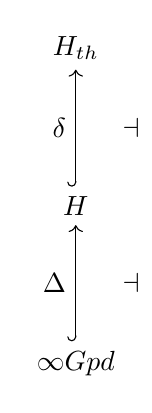
\begin{tikzpicture}
\node (H) at (0,2) {$H_{th}$};
\node (R) at (0,0) {$H$};
\node (G) at (0,-2) {$\infty Gpd$};

\draw[right hook->] [transform canvas={xshift = -100}] (R) -- (H) node[midway,left] {$\rho$};
\path [transform canvas={xshift = -80}] (R) -- (H) node[midway] {$\dashv$};
\draw[->] [transform canvas={xshift = -50}] (H) -- (R) node[midway,left] {$\pi$};
\path [transform canvas={xshift = -30}] (R) -- (H) node[midway] {$\dashv$};
\draw[right hook->] [transform canvas={xshift = 0}] (R) -- (H) node[midway,left] {$\delta$};
\path [transform canvas={xshift = 20}] (R) -- (H) node[midway] {$\dashv$};
\draw[->] [transform canvas={xshift = 50}] (H) -- (R) node[midway,left] {$\gamma$};

\draw[->] [transform canvas={xshift = -50}] (R) -- (G) node[midway,left] {$\Pi$};
\path [transform canvas={xshift = -30}] (R) -- (G) node[midway] {$\dashv$};
\draw[right hook->] [transform canvas={xshift = 0}] (G) -- (R) node[midway,left] {$\Delta$};
\path [transform canvas={xshift = 20}] (R) -- (G) node[midway] {$\dashv$};
\draw[->] [transform canvas={xshift = 50}] (R) -- (G) node[midway,left] {$\Gamma$};
\path [transform canvas={xshift = 70}] (R) -- (G) node[midway] {$\dashv$};
\draw[right hook->] [transform canvas={xshift = 100}] (G) -- (R) node[midway,left] {$\nabla$};

\draw[right hook->] [transform canvas={xshift = 150}] (G) -- (H) node[midway,left] {$\rotdel$};
\end{tikzpicture}
}
\end{center}

This picture is flipped diagonally from what Max had on the board. Some intuition:
\begin{itemize}
\item $\rho$ ??? inclusion of the ``reduced" objects into the ``thickened'' topos.  The reduced objects already have smooth structure, but in the thickened topos, there are objects containing ``infinitesimal directions'' allowing us to access this smooth structure.
\item $\pi$ ??? identifies infinitesimally close points
\item $\delta$ ??? inclusion of ``coreduced" objects, where coreduced objects have trivial tangent spaces at all points
\item $\gamma$ ??? maps any manifold to its discrete set of points
\item $\Pi$ takes the fundamental $\infty$-groupoid of a cohesive space
\item $\Delta$ equips a space with the discrete topology
\item $\Gamma$ forgets the cohesive structure
\item $\nabla$ equips a space with the codiscrete topology.
\end{itemize}
The modalities on $H_{th}$ are defined by:
\begin{itemize}
\item $\Red :\equiv \rho\pi$ and $\Cored :\equiv \delta\pi$ and $\Wat :\equiv \delta\gamma$, and we have $\Red \dashv \Cored \dashv \Wat$
\item $\shape :\equiv \delta \Delta \Pi \pi$ and $\flat :\equiv \delta \Delta \Gamma \gamma$ and $\sharp :\equiv \rotdel \Gamma \gamma$??? As in cohesion we should have $\shape \dashv \flat \dashv \sharp$
\end{itemize}
Remember that $\Cored$, $\shape$ and $\sharp$ are monadic and $\Red$, $\Wat$ and $\flat$ are comonadic. We think that:
\begin{itemize}
\item Every functor preserves products (as right adjoints, and by assumption for $\rho$ and $\Pi$)
\item Every upwards functor is fully faithful, which implies $\pi\rho = \pi\delta = 1_H$ and $\Gamma\Delta = \Gamma\nabla = 1_{\infty Gpd}$
\item Both $\shape$ and $\sharp$ land in the same subtopos, the ``discrete'' types. Both $\Cored$ and $\Wat$ land in the same subtopos, the ``coreduced'' types, and ``discrete'' $\subset$ ``coreduced''
\item $\sharp$ and $\Cored$ are both left exact (as composites of right adjoints), so are $\Wat$ and $\flat$
\item NEW: $\rho \Delta = \delta \Delta$ and $\Gamma\pi = \Gamma\gamma$, by the argument that $\rho, \delta$ and $\Delta$ are left adjoints, so preserve colimits, and also preserve the terminal object, but $\infty Gpd$ ``is the free cocompletion of its terminal object''.
\end{itemize} 
Lots of relations. The ones marked by ? I think cannot be expressed through other modalities.
\begin{align*}
    \Red \Cored = \Red && \Cored \Red = \Cored && \Cored \Wat = \Wat && \Wat \Cored = \Cored && \Red \Wat = ? && \Wat \Red = ? \\
    \flat \shape = \shape && \shape \flat = \flat && \sharp \flat = \sharp && \flat \sharp = \flat && \shape \sharp = ? && \sharp \shape = ? \\
    \Red \shape = ? && \shape \Red = \shape && \Red \flat = ? && \flat \Red = ? && \Red \sharp = ? && \sharp \Red = ? \\
    \Cored \shape = \shape && \shape \Cored = \shape && \Cored \flat = \flat && \flat \Cored = ? && \Cored \sharp = ? && \sharp \Cored = ? \\
    \Wat \shape = \shape && \shape \Wat = ? && \Wat \flat = \flat && \flat \Wat = \flat && \Wat \sharp = ? && \sharp \Wat = \sharp
\end{align*}
If we assume NEW too, we get more:
\begin{align*}
    \Red \Cored = \Red && \Cored \Red = \Cored && \Cored \Wat = \Wat && \Wat \Cored = \Cored && \Red \Wat = ? && \Wat \Red = ? \\
    \flat \shape = \shape && \shape \flat = \flat && \sharp \flat = \sharp && \flat \sharp = \flat && \shape \sharp = ? && \sharp \shape = ? \\
    \Red \shape = \color{red}{\shape} && \shape \Red = \shape && \Red \flat = \color{red}{\flat} && \flat \Red = \color{red}{\flat} && \Red \sharp = ? && \sharp \Red = \color{red}{\sharp} \\
    \Cored \shape = \shape && \shape \Cored = \shape && \Cored \flat = \flat && \flat \Cored = \color{red}{\flat} && \Cored \sharp = ? && \sharp \Cored = \color{red}{\sharp} \\
    \Wat \shape = \shape && \shape \Wat = ? && \Wat \flat = \flat && \flat \Wat = \flat && \Wat \sharp = ? && \sharp \Wat = \sharp
\end{align*}
We expect:
\begin{itemize}
\item $\Red D^1 \simeq 1$
\item $\Red \R \simeq \R$, and for any smooth manifold $\Red M \simeq M$
\item $\Cored D^1 \simeq 1$
\item $\Cored \R$ is not $\R$
\item The tangent spaces of any $\Cored X$ are trivial
\item Maps from $\Cored \R$ to $\R$ are constant
\item For any manifold $\Wat M\simeq\flat M$
\item Discrete spaces are reduced and coreduced
\item $A$ is coreduced if and only if for all $B$ there is a unique extension of any map $\varphi\colon \Red(B)\to A$ along the counit of $\Red$:
\begin{center}
    \begin{tikzpicture}[node distance=2.3cm, auto]

    \node (RB) {$\Red(B)$};
    \node[below of=RB] (B) {$B$};
    \node[right of=RB] (A) {$A$};

    \draw[->] (RB) to (B);
    \draw[->] (RB) to node {$\varphi$} (A);
    \draw[->, dashed] (B) to (A); 

    \end{tikzpicture}
\end{center}
\end{itemize}
For the model $\mathrm{FSSet}_1$ (formal smooth sets of order one) of sheaves on $\{\R^n\times (D^1)^m \}$,
the modalities are given by
\begin{itemize}
\item $\Red(\R^n\times (D^1)^m)=\R^n$ for the representables $\R^n\times (D^1)^m\in\mathrm{FSSet}_1$
\item $\Cored(F)(\R^n\times (D^1)^m)=F(\R^n)$
\item $\Wat(F)(\R^n\times (D^1)^m)=\mathrm{FSSet}_1(\Cored(\R^n\times(D^1)^m), F)$
\end{itemize}

\newpage
\section{A type theory for $\Wat$ and $\flat$}

How contexts work:
\begin{mathpar}
\inferrule*{ }{\cdot \ctx} \and
\inferrule*{\Gamma \ctx \and \Gamma \cbar \cdot \cbar \cdot \yields A \type}{\Gamma, x : A \ctx} \\
\inferrule*{\Gamma \ctx}{\Gamma \cbar \cdot \ctx} \and
\inferrule*{\Gamma \cbar \Delta \ctx \and \Gamma \cbar \Delta \cbar \cdot \yields A \type}{\Gamma \cbar \Delta, x : A \ctx} \\
\inferrule*{\Gamma \cbar \Delta \ctx}{\Gamma \cbar \Delta \cbar \cdot \ctx} \and
\inferrule*{\Gamma \cbar \Delta \cbar \Theta \ctx \and \Gamma \cbar \Delta \cbar \Theta \yields A \type}{\Gamma \cbar \Delta \cbar \Theta, x : A \ctx}
\end{mathpar}
Substitution principles:
\begin{mathpar}
\inferrule*{\Gamma \cbar \cdot\cbar \cdot \yields e : A \\ \Gamma, x ::: A, \Gamma' \cbar \Delta \cbar \Theta \yields e' : B}{\Gamma, \Gamma'[e/x] \cbar \Delta[e/x] \cbar \Theta[e/x] \yields e'[e/x] : B [e/x]} \\
\inferrule*{\Gamma \cbar \Delta \cbar \cdot \yields e : A \\ \Gamma \cbar \Delta, x :: A, \Delta' \cbar \Theta \yields e' : B}{\Gamma \cbar \Delta, \Delta'[e/x] \cbar \Theta[e/x] \yields e'[e/x] : B [e/x]} \\
\inferrule*{\Gamma \cbar \Delta \cbar \Theta \yields e : A \\ \Gamma \cbar \Delta \cbar \Theta, x : A , \Theta' \yields e' : B}{\Gamma \cbar \Delta \cbar \Theta, \Theta'[e/x] \yields e'[e/x] : B [e/x]}
\end{mathpar}
Flat:
\begin{mathpar}
\inferrule*{\Gamma \cbar \cdot \cbar \cdot \yields A \type}{\Gamma \cbar \Delta \cbar \Theta \yields \flat A \type} \\
\inferrule*{\Gamma \cbar \cdot \cbar \cdot \yields a : A}{\Gamma \cbar \Delta \cbar \Theta \yields a^\flat : \flat A} \and 
\inferrule*{\Gamma \cbar \Delta \cbar \Theta, u : \flat A \yields B \type \\\\
\Gamma \cbar \Delta \cbar \Theta \yields e : \flat A \\ \Gamma, x ::: A \cbar \Delta \cbar \Theta \yields e' : B[x^\flat/u]}{\Gamma \cbar \Delta \cbar \Theta \yields (\flatletin{x}{e}{e'}) : B[e/u]} \\
\inferrule*{\Gamma \cbar \Delta, u :: \flat A \cbar \cdot \yields C \type \\\\
\Gamma \cbar \Delta \cbar \cdot \yields e : \flat A \\ 
\Gamma, x ::: A \cbar \Delta \cbar \cdot \yields e' : C[x^\flat/u]}{\Gamma \cbar \Delta \cbar \Theta \yields \coredflatind{x}{e}{e'} : C[e/u]} \\
\inferrule*{\Gamma, u ::: \flat A \cbar \cdot \cbar \cdot \yields C \type \\\\ 
\Gamma \cbar \cdot \cbar \cdot \yields e : \flat A \\ 
\Gamma, x ::: A \cbar \cdot \cbar \cdot \yields e' : C[x^\flat/u]}{\Gamma \cbar \Delta \cbar \Theta \yields \crispflatind{x}{e}{e'} : C[e/u]} \\
\end{mathpar}
Seems like the 3 $\flat$ ind principles can be abstracted into one easily by putting a partial order on the contexts

\newpage
\section{A simple type theory for $\shape$, $\flat$ and $\sharp$}
\label{sec:cohesive}

Mode theory: I changed the names of the 1-morphisms to $s$ for shapely and $c$ for crisp
\begin{center}
  \begin{tabular}{| l | l |}
    \hline
    0 & $p$ \\
    \hline
    1 & \pbox{20cm}{
      $s : p \to p$ and $c : p \to p$ \\
      and a product that the above respect \\
      $\times : (p, p) \to p$ \hspace{2ex} $\top : () \to p$
    }\\
    \hline
    2 & $unit : 1_p \Rightarrow s$ \hspace{2ex} $counit : c \Rightarrow 1_p$ \\
    \hline
     eq & \pbox{20cm}{\vspace{1ex}
       $s \circ s = s$ \\
       $c \circ c = c$ \\
       $s \circ c = c$ \\
       $c \circ s = s$ \\
       (the inner one always wins) \\
        and all the expected triangle equations
    }\\
    \hline
  \end{tabular}
\end{center}
We then define $\shape := F_s$, either $\flat := F_c$ or $\flat := U_s$ and $\sharp := U_c$.

Context structure: For this simply typed case, our context descriptors can all be simplified and rearranged into the form $c(x_1) , \dots , c(x_n) , y_1 , \dots , y_m , s(z_1) , \dots , s(z_o)$. We therefore write our judgments as $\Gamma \cbar \Delta \cbar \Theta \yields A$, where this time $\Gamma$ is the crisp context, $\Delta$ is the ordinary context and $\Theta$ is the shapely context.\\
The spatial intuition is that a term $\Gamma\cbar\Delta\cbar\Theta\yields a : A$ denotes a function $a : \Gamma\times\Delta\times\Theta\to A$ that is continuous in $\Delta$ and locally constant in $\Theta$ (i.e. constant on each connected component). More generally, it is a continuous function $\flat\Gamma\times\Delta\times\shape\Theta \to A$. This gives us a natural ordering: locally constant is stronger than continuous is stronger than discontinuous, so when given a choice in a typing rule we should use the strongest for a conclusion and the weakest for a premise. This gives intuition for the structural rules

Structural rules:
\begin{mathpar}
\inferrule*{\Gamma \cbar \Delta \cbar \Theta, x:A \yields B}{\Gamma \cbar \Delta, x:A \cbar \Theta \yields B} \and
\inferrule*{\Gamma \cbar \Delta, x:A \cbar \Theta \yields B}{\Gamma, x:A \cbar \Delta \cbar \Theta \yields B}
\end{mathpar}
Variable rules (can't use a shapely var directly!):
\begin{mathpar}
\inferrule*{~}{\Gamma,x:A \cbar \Delta \cbar \Theta \yields x : A}\and
\inferrule*{~}{\Gamma \cbar \Delta,x:A \cbar \Theta \yields x : A}
\end{mathpar}
Cut principles:
\begin{mathpar}
\inferrule*{\Gamma \cbar \cdot \cbar \Theta \yields A \\ \Gamma, x:A \cbar \Delta \cbar \Theta \yields C}{\Gamma \cbar \Delta \cbar \Theta \yields C} \and
\inferrule*{\Gamma \cbar \Delta \cbar \Theta \yields A \\ \Gamma \cbar \Delta, x : A \cbar \Theta \yields C}{\Gamma \cbar \Delta \cbar \Theta \yields C} \and
\inferrule*{\Gamma \cbar \Theta \cbar \cdot \yields A \\ \Gamma \cbar \Delta \cbar \Theta, x : A \yields C}{\Gamma \cbar \Delta \cbar \Theta \yields C}
\end{mathpar}
Rules for $\sharp$:
\begin{mathpar}
\inferrule*{\Gamma, \Delta \cbar \cdot \cbar \Theta \yields A}{\Gamma \cbar \Delta \cbar \Theta \yields \sharp A} \and
\inferrule*{\Gamma, x : A \cbar \Delta \cbar \Theta \yields C}{\Gamma, x : \sharp A \cbar \Delta \cbar \Theta \yields C}
\end{mathpar}
Rules for $\flat$ as an $F$-type.
\begin{mathpar}
\inferrule*{\Gamma \cbar \cdot \cbar \Theta \yields A}{\Gamma \cbar \Delta \cbar \Theta \yields \flat A} \and
\inferrule*{x : \flat A \in \Gamma \cbar \Delta \cbar \Theta \\ \Gamma, y : A \cbar \Delta \cbar \Theta \yields C}{\Gamma \cbar \Delta \cbar \Theta \yields C} 
\end{mathpar}
Rules for $\flat$ as a $U$-type.
\begin{mathpar}
\inferrule*{\Gamma \cbar \cdot \cbar \Delta, \Theta \yields A}{\Gamma \cbar \Delta \cbar \Theta \yields \flat A} \and
\inferrule*{\Gamma, x : A \cbar \Delta \cbar \Theta \yields C}{\Gamma \cbar \Delta \cbar \Theta, x : \flat A \yields C} 
\end{mathpar}
Conjecture: that UL-rule is equivalent to either of the following natural deduction style rules:
\begin{mathpar}
\inferrule*{\Gamma \cbar \Delta \cbar \Theta \yields \flat A}{\Gamma \cbar \cdot \cbar \Delta, \Theta \yields A} \and
\inferrule*{\Gamma \cbar \Theta \cbar \cdot \yields \flat A}{\Gamma \cbar \Delta \cbar \Theta \yields A}
\end{mathpar}
Rules for $\shape$: 
\begin{mathpar}
\inferrule*{\Gamma \cbar \Delta, \Theta \cbar \cdot \yields A}{\Gamma \cbar \Delta \cbar \Theta \yields \shape A} \and
\inferrule*{x : \shape A \in \Gamma \cbar \Delta \cbar \Theta \\ \Gamma \cbar \Delta \cbar \Theta, y : A \yields C}{\Gamma \cbar \Delta \cbar \Theta \yields C} 
\end{mathpar}

Conjecture: for the mode theory of a product preserving adjunction, show that the middle F and U line up.

\newpage
\section{A simple type theory for $\Red$, $\Cored$ and $\Wat$}
\label{sec:differential}

Mode theory:
\begin{center}
  \begin{tabular}{| l | l |}
    \hline
    0 & $p$ \\
    \hline
    1 & \pbox{20cm}{
      $r : p \to p$ and $i : p \to p$ \\
      and a product that the above respect \\
      $\times : (p, p) \to p$ \hspace{2ex} $\top : () \to p$
    }\\
    \hline
    2 & $unit : 1_p \Rightarrow i$ \hspace{2ex} $counit : r \Rightarrow 1_p$ \\
    \hline
     eq & \pbox{20cm}{\vspace{1ex}
       $r \circ r = r$ \\
       $i \circ i = i$ \\
       $r \circ i = r$ \\
       $i \circ r = i$ \\
       (the outer one always wins) \\
       and all the expected triangle equations
    }\\
    \hline
  \end{tabular}
\end{center}

We then define $\Red := F_r$, either $\Cored := F_i$ or $\Cored := U_r$ and $\Wat := U_i$.

Structural Rules:
\begin{mathpar}
  \inferrule*
  {\Gamma \mid \Delta \mid \Theta,x:A \vdash C}
  {\Gamma \mid \Delta,x:A \mid \Theta \vdash C}
\and
  \inferrule*
  {\Gamma \mid \Delta,x:A \mid \Theta \vdash C}
  {\Gamma,x:A \mid \Delta \mid \Theta \vdash C}
\end{mathpar}

Variable Rules:
\begin{mathpar}
  \inferrule*
  {~}
  {\Gamma,x:A \mid \Delta \mid \Theta \vdash A}
\and 
  \inferrule*
  {~}
  {\Gamma \mid \Delta,x:A \mid \Theta \vdash A}
\end{mathpar}

Cut rules:
\begin{mathpar}
  \inferrule*
  {\Gamma \mid \cdot \mid \cdot \vdash A
  \\
   \Gamma,x:A \mid \Delta \mid \Theta \vdash C}
  {\Gamma \mid \Delta \mid \Theta \vdash C}
\and 
  \inferrule*
  {\Gamma \mid \Delta \mid \Theta \vdash A
  \\
   \Gamma \mid \Delta,x:A \mid \Theta \vdash C}
  {\Gamma \mid \Delta \mid \Theta \vdash C}
\and 
  \inferrule*
  {\Theta \mid \cdot \mid \cdot \vdash A \\
   \Gamma \mid \Delta \mid \Theta,x:A \vdash C}
  {\Gamma \mid \Delta \mid \Theta \vdash C}
\end{mathpar}

% \Gamma \cbar \Delta \cbar \Theta \yields A
Rules for $\Red$:
\begin{mathpar}
\inferrule*{x : \Red A \in \Gamma \cbar \Delta \\ \Gamma, y : A \cbar \Delta \cbar \Theta \yields C}{\Gamma \cbar \Delta \cbar \Theta \yields C} \and
\inferrule*{\Gamma \cbar \Delta \cbar \Theta, x : A \yields C}{\Gamma \cbar \Delta \cbar \Theta, x : \Red A \yields C} \\
\inferrule*{\Gamma \cbar \cdot \cbar \cdot \yields A}{\Gamma \cbar \Delta \cbar \Theta \yields \Red A}
\end{mathpar}
Rules for $\Cored$ as an $F$:
\begin{mathpar}
\inferrule*{\Gamma, y : A \cbar \Delta \cbar \Theta \yields C}{\Gamma, x : \Cored A \cbar \Delta \cbar \Theta \yields C} \and
\inferrule*{x : \Cored A \in \Delta \cbar \Theta \\ \Gamma \cbar \Delta \cbar \Theta, x : A \yields C}{\Gamma \cbar \Delta \cbar \Theta \yields C} \\
\inferrule*{\Gamma, \Delta, \Theta \cbar \cdot \cbar \cdot \yields A}{\Gamma \cbar \Delta \cbar \Theta \yields \Cored A}
\end{mathpar}
Rules for $\Cored$ as a $U$:
\begin{mathpar}
\inferrule*{\Gamma, y : A \cbar \Delta \cbar \Theta \yields C}{\Gamma, x : \Cored A \cbar \Delta \cbar \Theta \yields C} \and
\inferrule*{\Gamma, \Delta, \Theta \cbar \cdot \cbar \cdot \yields A}{\Gamma \cbar \Delta \cbar \Theta \yields \Cored A}
\end{mathpar}
Rules for $\Wat$:
\begin{mathpar}
\inferrule*{\Gamma, \Delta, \Theta \cbar \cdot \cbar \cdot  \yields \Wat A}{\Gamma \cbar \Delta \cbar \Theta \yields A} \and
\inferrule*{\cdot \cbar \cdot \cbar \Gamma, \Delta, \Theta  \yields A}{\Gamma \cbar \Delta \cbar \Theta \yields \Wat A}
\end{mathpar}

\newpage
\section{Adding dependent types to \cref{sec:cohesive}}
\label{sec:dependent-cohesive}

Dependency rules:
\begin{enumerate}
    \item $\flat$ can only depend on discrete things
    \item $\sharp$ can only depend on discrete things (although it can promote to discrete)
    \item $\shape$ can depend on anything
    \item Discrete things include crisp and shapely things
\end{enumerate}


\begin{align}
  m &::= c \mid 1 \mid s \\
  \Gamma &::= \cdot \mid \Gamma,x:_m A
\end{align}

Context well-formedness $\Gamma \ctx$:
\begin{mathpar}
    \inferrule*{~}{\cdot \ctx} 
    \and 
    \inferrule*{\Gamma \ctx \\ \Gamma|_m \vdash A \type}
               {\Gamma,x:_m A \ctx}
\end{mathpar}

Context restriction $\Gamma |_m$:
\begin{align*}
    \Gamma|_1 &= \Gamma|_s = \Gamma \\
    \cdot |_c &= \cdot \\
    (\Gamma,x:_1 A)|_c &= \Gamma|_c \\
    (\Gamma,x:_c A)|_c &= \Gamma|_c, x:_c A \\
    (\Gamma,x:_s A)|_c &= \begin{cases} 
                            \Gamma|_c,x:_s A &\text{if}~\Gamma|_c \vdash A \type \\
                            \Gamma|_c &\text{otherwise}
                         \end{cases}
\end{align*}

Flat promotion $\flat\Gamma$:
\begin{align*}
    \flat(\cdot) &:= \cdot \\
    \flat(\Gamma,x:_m A) &= \flat \Gamma, x:_{\flat(m)} A \\
    \flat(c) &= c \\
    \flat(1) &= c \\
    \flat(s) &= s
\end{align*}

Unshape operation $\unshape(\Gamma)$:
\begin{align*}
    \unshape(\cdot) &= \cdot \\
    \unshape(\Gamma,x:_m A) &= \unshape(\Gamma),x:_{\unshape(m)} A \\
    \unshape(c) &= c \\
    \unshape(1) &= 1 \\
    \unshape(s) &= 1
\end{align*}
{\color{red}{The resulting context is not necessarily well-formed, e.g. $x:_s A,y:_c B[x]$. This is a problem with this entire section.}}

Type well-formedness $\Gamma \vdash A \type$
\begin{mathpar}
    \inferrule*
    {\Gamma|_c \vdash A \type}
    {\Gamma \vdash \flat A \type}
\and 
    \inferrule*
    {\flat\Gamma \vdash A \type}
    {\Gamma \vdash \sharp A \type}
\and 
    \inferrule*
    {\Gamma \vdash A \type}
    {\Gamma \vdash \shape A \type}
\end{mathpar}

Term judgment shorthand $\Gamma \vdash_m e : A$:
\begin{align*}
    \Gamma \vdash_1 e : A &:= \Gamma \vdash e : A \\
    \Gamma \vdash_c e : A &:= \Gamma|_c \vdash e : A \\
    \Gamma \vdash_s e : A &:= \unshape(\Gamma|_c) \vdash e : A
\end{align*}

\subsection{Term judgments $\Gamma \vdash e : A$}

Variable and cut
\begin{mathpar}
  \inferrule*
  {x:_m A \in \Gamma  \\ m \in \{c,1\}}
  {\Gamma \vdash x : A}
\and 
    \inferrule*
    {\Gamma \vdash_m e' : A \\
     \Gamma,x:_m A, \Gamma' \vdash e : C}
    {\Gamma,\Gamma'[e'/x] \vdash e[e'/x] : C[e'/x]}
\end{mathpar}

$\flat$ rules:
\begin{mathpar}
  \inferrule*
  {\Gamma|_c \vdash e : A}
  {\Gamma \vdash e^\flat : \flat A}
\and 
    \inferrule*
    {\Gamma,x:_m \flat A \vdash C \type \\
     \Gamma \vdash e : \flat A \\
     \Gamma,y:_c A \vdash e' : C[y^\flat / x]}
    {\Gamma \vdash \flatletin{y}{e}{e'} : C[e/x]}
\end{mathpar}

$\sharp$ rules:
\begin{mathpar}
    \inferrule*
    {\flat \Gamma \vdash e : A}
    {\Gamma \vdash e^\sharp : \sharp A}
\and 
    \inferrule*
    {\Gamma|_c \vdash e : \sharp A}
    {\Gamma \vdash e_\sharp : A}
\end{mathpar}

$\shape$ rules. Unshape is problematic.
\begin{mathpar}
    \inferrule*
    {\unshape (\Gamma) \vdash e : A}
    {\Gamma \vdash e^{\shape} : \shape A}
  \and 
    \inferrule*
    {\Gamma,x:_m\shape A \vdash C \type \\
     \Gamma \vdash_m e : \shape A \\
     \Gamma,y:_{\shape} A \vdash C[y^{\shape} / x]}
    {\Gamma \vdash \shapeletin{y}{e}{e'} : C[e/x]}
\end{mathpar}


\newpage
\section{A simple type theory for the kitchen sink}
\label{sec:differential-simple}

\begin{center}
  \begin{tabular}{| l | l |}
    \hline
    0 & $p$ \\
    \hline
    1 & \pbox{20cm}{\vspace{0.5ex}
      $r,i,s,c : p \to p$ \\
      and a product that the above respect \\
      $\times : (p, p) \to p$ \hspace{2ex} $\top : () \to p$
    }\\
    \hline
    2 & $c \Rightarrow r \Rightarrow 1 \Rightarrow i \Rightarrow s$ \\
    \hline
     eq & \pbox{20cm}{\vspace{1ex}
       $mc = c$ \\
       $ms = s$ \\
       $mi = m$ \\
       $mr = m$ \vspace{1ex}
    }\\
    \hline
  \end{tabular}
\end{center}
The contexts look like $\Gamma \cbar \Delta \cbar \Theta \cbar \Lambda \cbar \Xi$ where in order these are cr1is. We might also just annotate variables $x :_m A$ to say $x$ is in mode $m$.

Variable rule:
\begin{mathpar}
\inferrule*{m \in \{c,r,1\} \and x :_m A \in \Gamma}{\Gamma \yields x : A}
\end{mathpar}

The structural rules are similar to before: you can move a variable to the left if you want (going downwards). In particular, the following structural rule should be admissible:
\begin{mathpar}
    \inferrule*
    {m \Rightarrow n \\ \Gamma,x:_n A \vdash e : B}
    {\Gamma,x:_m A \vdash e : B}
\end{mathpar}
In what follows, the rules in quotes are the ones that don't build in the structural rules.

Define:
\begin{align*}
    \Gamma \cbar \Delta \cbar \Theta \cbar \Lambda \cbar \Xi \yields^c A &:\equiv \Gamma \cbar \cdot \cbar \cdot \cbar \cdot \cbar \Xi \yields A \\
    \Gamma \cbar \Delta \cbar \Theta \cbar \Lambda \cbar \Xi \yields^r A &:\equiv \Gamma \cbar \Delta \cbar \cdot \cbar \cdot \cbar \Xi \yields A \\
    \Gamma \cbar \Delta \cbar \Theta \cbar \Lambda \cbar \Xi \yields^1 A &:\equiv \Gamma \cbar \Delta \cbar \Theta \cbar \Lambda \cbar \Xi \yields A \\
    \Gamma \cbar \Delta \cbar \Theta \cbar \Lambda \cbar \Xi \yields^i A &:\equiv \Gamma \cbar \Lambda \cbar \cdot \cbar \cdot \cbar \Xi \yields A \\
    \Gamma \cbar \Delta \cbar \Theta \cbar \Lambda \cbar \Xi \yields^s A &:\equiv \Gamma \cbar \Xi \cbar \cdot \cbar \cdot \cbar \cdot \yields A 
\end{align*}

Then we can express cut as:
\begin{mathpar}
\inferrule*{\Gamma \yields^m e : A \\ \Gamma, x :_m A \yields e' : C}{\Gamma \yields e'[e/x] : C}
\end{mathpar}
Rules for $\Red$: Notice that the hypothesis of $\Red$E varies universally over $m$. This can be split into two rules, $m=1$, when $mr=r$, and $m \neq 1$, when $mr = m$.
\begin{mathpar}
\inferrule*[Right = ``$\Red$I'']{\Gamma \yields^r e : A}{\Gamma \yields e^\Red : \Red A} \and
\inferrule*[Right = $\Red$I]{\Gamma \cbar \Delta \cbar \cdot \cbar \Theta, \Lambda \cbar \Xi \yields e : A}{\Gamma \cbar \Delta \cbar \Theta \cbar \Lambda \cbar \Xi \yields e^\Cored : \Cored A} \and
\inferrule*[Right = $\Red$E]{\Gamma \yields^m e : \Red A \and \Gamma, x:_{mr} A \yields e' : C}{\Gamma \yields \redind{x}{m}{e}{e'} : C}
\end{mathpar}
Rules for $\Cored$: Notice that the hypothesis of $\Cored$E varies universally over $m$. This can be split into two rules, $m=1$, when $mi=i$, and $m \neq 1$, when $mi = m$.
\begin{mathpar}
\inferrule*[Right = ``$\Cored$I'']{\Gamma \yields^i e : A}{\Gamma \yields e^\Cored : \Cored A} \and
\inferrule*[Right = $\Cored$I]{\Gamma \cbar \Delta, \Theta, \Lambda \cbar \cdot \cbar \cdot \cbar \Xi \yields e : A}{\Gamma \cbar \Delta \cbar \Theta \cbar \Lambda \cbar \Xi \yields e^\Cored : \Cored A} \and
\inferrule*[Right = $\Cored$E]{\Gamma \yields^m e : \Cored A \and \Gamma, x:_{mi} A \yields e' : C}{\Gamma \yields \coredind{x}{m}{e}{e'} : C}
\end{mathpar}
Rules for $\Wat$:
\begin{mathpar}
\inferrule*[Right = $\Wat$I]{\Gamma \cbar \cdot \cbar \cdot \cbar \Delta, \Theta, \Lambda \cbar \Xi \yields e : A}{\Gamma \cbar \Delta \cbar \Theta \cbar \Lambda \cbar \Xi \yields e^\Wat : \Wat A} \and
\inferrule*[Right = ``$\Wat$E'']{\Gamma \yields^i  e : \Wat A}{\Gamma \yields e_\Wat : A} \and
\inferrule*[Right = $\Wat$E]{\Gamma \cbar \Delta, \Theta, \Lambda \cbar \cdot \cbar \cdot \cbar \Xi \yields e : \Wat A}{\Gamma \cbar \Delta \cbar \Theta \cbar \Lambda \cbar \Xi \yields e_\Wat : A}
\end{mathpar}
Rules for $\shape$:
\begin{mathpar}
\inferrule*[Right = ``$\shape$I'']{\Gamma \yields^s e : A}{\Gamma \yields e^{\shape} : \shape A} \and
\inferrule*[Right = $\shape$I]{\Gamma \cbar \Delta, \Theta, \Lambda, \Xi \cbar \cdot \cbar \cdot \cbar \cdot \yields e : A}{\Gamma \cbar \Delta \cbar \Theta \cbar \Lambda \cbar \Xi \yields e^{\shape} : \shape A} \and
\inferrule*[Right = ``$\shape$E'']{\Gamma \yields^m e : \shape A \and \Gamma, x:_s A \yields e' : C}{\Gamma \yields \coredind{x}{m}{e}{e'} : C} \and
    \inferrule*[Right=$\shape$E]
    {\Gamma \mid \Delta,\Theta,\Lambda,\Xi \mid \cdot \mid \cdot \mid \cdot \vdash e : \shape A \\
     \Gamma \mid \Delta \mid \Theta \mid \Lambda \mid \Xi,x:A \vdash e' : C}
    {\Gamma \mid \Delta \mid \Theta \mid \Lambda \mid \Xi \vdash \shapeletin{x}{e}{e'} : C}
\end{mathpar}
Rules for $\flat$:
\begin{mathpar}
\inferrule*[Right = ``$\flat$I'']{\Gamma \yields^c e : A}{\Gamma \yields e^\flat : \flat A} \and
\inferrule*[Right = $\flat$I]{\Gamma \cbar \cdot \cbar \cdot \cbar \cdot \cbar \Delta, \Theta, \Lambda, \Xi \yields e : A}{\Gamma \cbar \Delta \cbar \Theta \cbar \Lambda \cbar \Xi \yields e^\flat : \flat A} \and
\inferrule*[Right = ``$\flat$E'']{\Gamma, \yields^m e : \flat A \and \Gamma x :_c A \yields e' : C}{\Gamma \yields \flatind{x}{m}{e}{e'} : C}
\and 
\inferrule*[Right = $\flat$E]
           {\Gamma \mid \Delta,\Theta,\Lambda,\Xi \mid \cdot \mid \cdot \mid \cdot \vdash e : \flat A \\
            \Gamma,x:A \mid \Delta \mid \Theta \mid \Lambda \mid \Xi \vdash e' : C}
           {\Gamma \mid \Delta \mid \Theta \mid \Lambda \mid \Xi \vdash \flatletin{x}{e}{e'} : C}
\end{mathpar}
Rules for $\sharp$: 
\begin{mathpar}
\inferrule*[Right = $\sharp$I]{\Gamma, \Delta, \Theta, \Lambda \cbar \cdot \cbar \cdot \cbar \cdot \cbar \Xi \yields e : A}{\Gamma \cbar \Delta \cbar \Theta \cbar \Lambda \cbar \Xi \yields e^\sharp : \sharp A} \and
\inferrule*[Right = ``$\sharp$E'']{\Gamma \yields^c e : \sharp A}{\Gamma \yields e_\sharp : A} \and
\inferrule*[Right = $\sharp$E]{\Gamma \cbar \cdot \cbar \cdot \cbar \cdot \cbar \Delta, \Theta, \Lambda, \Xi \yields e : \sharp A}{\Gamma \cbar \Delta \cbar \Theta \cbar \Lambda \cbar \Xi \yields e_\sharp : A} 
\end{mathpar}

Things to prove:

(commented out -- please format)

%I think this answers a question that came up today:
%https://nforum.ncatlab.org/discussion/7811/differential-cohesion/?Focus=63239#Comment_63239
%I expect the corresponding type-theoretic result (discrete types are
%reduced, I think) should be provable once you have a dependent type
%theory with all the differential-cohesion modalities.  (-:O

%Actually, I don't think this needs all the modalities: all it needs is
%that R is an idempotent comonad that can depend on crisp things.
%Here's an informal version of the internal argument.

%Let X be discrete.  It suffices to construct a section X -> RX of the
%counit RX -> X.  Thus, assume x:X and we want to define a point of RX.
%Since X is discrete, the assumption x:X may as well be crisp.  But now
%our context is entirely crisp and R can be formed in crisp context, so
%R-intro tells us that we can get a point of RX from a point of X ---
%which we have.  And R-comp implies that this point maps down to x in
%X, so by crisp Id-induction the composite X -> RX -> X is the
%identity.

\end{document}